\section{Cours 8}\label{cours-8}

\subsection{Rappel}\label{rappel}

On se souvient que l'accès à une variable partagée doit être protégée.
soit via: - Mutex: \texttt{lock()} et \texttt{unlock()} - Sémaphore:
\texttt{wait()} et \texttt{post()}

\subsection{Problème d'exclusion
fondamentale}\label{probluxe8me-dexclusion-fondamentale}

\subsubsection{Résultat Théorique}\label{ruxe9sultat-thuxe9orique}

il est impossible de réaliser un algorithme d'exclusion mutuelle pour N
threads avec moins de N valeurs partagées si on utilise uniquement des
opérations de lecture et d'écriture.

\subsubsection{Essais et Erreurs}\label{essais-et-erreurs}

\paragraph{Les bases}\label{les-bases}

Si on a 2 threads qui doivent accéder à une section critique, il faut
garantir: - La \emph{Safety}: ils ne vont pas y accéder de manière
conjointe - La \emph{Liveness}: ils doivent y accéder en un temps fini.

\paragraph{Premier Essai}\label{premier-essai}

On peut utiliser une variable \texttt{turn} qui indique l'envie d'un
thread d'arriver en zone critique.

\begin{Shaded}
\begin{Highlighting}[]
\CommentTok{// thread 1 }
\ControlFlowTok{while} \OperatorTok{(}\NormalTok{turn}\OperatorTok{!=}\DecValTok{0}\OperatorTok{)} \OperatorTok{\{} 
    \CommentTok{/* loop */} 
\OperatorTok{\}} 
\NormalTok{section\_critique}\OperatorTok{();}
\NormalTok{turn}\OperatorTok{=}\DecValTok{1}\OperatorTok{;}

\CommentTok{// thread 2 }
\ControlFlowTok{while} \OperatorTok{(}\NormalTok{turn}\OperatorTok{!=}\DecValTok{1}\OperatorTok{)} \OperatorTok{\{}
    \CommentTok{/* loop */} 
\OperatorTok{\}} 
\NormalTok{section\_critique}\OperatorTok{();}
\NormalTok{turn}\OperatorTok{=}\DecValTok{0}\OperatorTok{;}
\end{Highlighting}
\end{Shaded}

On respecte bien l'exclusion mutuelle puisque pour que les deux threads
s'exécutent simultanément, il faudrait que \texttt{turn\ =\ 1} et en
même temps \texttt{turn\ =\ 0}.

Mais pour la \textbf{liveness}, si le thread 1 a fini de s'exécuter et
qu'il veut ré-exécuter il ne pourra pas le faire tant que le premier
thread ne s'exécute ce qui est problématique.

\begin{itemize}
\tightlist
\item
  \textbf{Safety}: ✅
\item
  \textbf{Liveness}: ❌
\end{itemize}

\paragraph{Second Essai}\label{second-essai}

Ici, l'approche consiste à utiliser un tableau de \emph{flag} qui
indique si le thread veut s'exécuter. Donc une valeur de \texttt{1} à
l'emplacement 0 indique que le thread 1 veut s'exécuter.

\begin{Shaded}
\begin{Highlighting}[]
\CommentTok{// Thread A }
\ControlFlowTok{while} \OperatorTok{(}\NormalTok{flag}\OperatorTok{[}\NormalTok{B}\OperatorTok{]==}\KeywordTok{true}\OperatorTok{)} \OperatorTok{\{}
    \CommentTok{/* loop */} 
\OperatorTok{\}}
\NormalTok{flag}\OperatorTok{[}\NormalTok{A}\OperatorTok{]=}\KeywordTok{true}\OperatorTok{;}
\NormalTok{section\_critique}\OperatorTok{();}
\NormalTok{flag}\OperatorTok{[}\NormalTok{A}\OperatorTok{]=}\KeywordTok{false}\OperatorTok{;}

\CommentTok{// Thread B }
\ControlFlowTok{while} \OperatorTok{(}\NormalTok{flag}\OperatorTok{[}\NormalTok{A}\OperatorTok{]==}\KeywordTok{true}\OperatorTok{)} \OperatorTok{\{} 
    \CommentTok{/* loop */}
\OperatorTok{\}} 
\NormalTok{flag}\OperatorTok{[}\NormalTok{B}\OperatorTok{]=}\KeywordTok{true}\OperatorTok{;}
\NormalTok{section\_critique}\OperatorTok{();}
\NormalTok{flag}\OperatorTok{[}\NormalTok{B}\OperatorTok{]=}\KeywordTok{false}\OperatorTok{;}
\end{Highlighting}
\end{Shaded}

La \textbf{Liveness} est bien respecté car le thread A est seulement
bloqué si le thread B est dans session critique.

Les threads peuvent simultanément lire \texttt{flag{[}A{]}} et
\texttt{flag{[}B{]}} a \texttt{false} et sortir de leur zone critique.

\begin{itemize}
\tightlist
\item
  \textbf{Safety}: ❌
\item
  \textbf{Liveness}: ✅
\end{itemize}

\paragraph{Corriger le problème}\label{corriger-le-probluxe8me}

On peut déplacer l'assignation comme suit:

\begin{Shaded}
\begin{Highlighting}[]
\NormalTok{flag}\OperatorTok{[}\NormalTok{A}\OperatorTok{]=}\KeywordTok{true}\OperatorTok{;} 
\ControlFlowTok{while} \OperatorTok{(}\NormalTok{flag}\OperatorTok{[}\NormalTok{B}\OperatorTok{]==}\KeywordTok{true}\OperatorTok{)} \OperatorTok{\{} 
    \CommentTok{/* loop */} 
\OperatorTok{\}} 
\NormalTok{section\_critique}\OperatorTok{();}
\NormalTok{flag}\OperatorTok{[}\NormalTok{A}\OperatorTok{]=}\KeywordTok{false}\OperatorTok{;}
\end{Highlighting}
\end{Shaded}

On perd la propriété de \emph{Liveness} même si on retrouve celle de
\emph{safety}. Ils peuvent mutuellement se bloquer s'ils veulent tous
les deux s'exécuter.

\begin{itemize}
\tightlist
\item
  \textbf{Safety}: ✅
\item
  \textbf{Liveness}: ❌
\end{itemize}

\subsection{Algorithme de Peterson}\label{algorithme-de-peterson}

\begin{Shaded}
\begin{Highlighting}[]
\PreprocessorTok{\#define A }\DecValTok{0}\PreprocessorTok{ }
\PreprocessorTok{\#define B }\DecValTok{1}\PreprocessorTok{ }

\DataTypeTok{int}\NormalTok{ turn }\OperatorTok{=}\NormalTok{ A}\OperatorTok{;}
\DataTypeTok{int}\NormalTok{ flag}\OperatorTok{[];} 
\NormalTok{flag}\OperatorTok{[}\NormalTok{A}\OperatorTok{]=}\KeywordTok{false}\OperatorTok{;}
\NormalTok{flag}\OperatorTok{[}\NormalTok{B}\OperatorTok{]=}\KeywordTok{false}\OperatorTok{;}

\CommentTok{// thread A }
\NormalTok{flag}\OperatorTok{[}\NormalTok{A}\OperatorTok{]=}\KeywordTok{true}\OperatorTok{;} 
\NormalTok{turn}\OperatorTok{=}\NormalTok{B}\OperatorTok{;} 
\ControlFlowTok{while}\OperatorTok{((}\NormalTok{flag}\OperatorTok{[}\NormalTok{B}\OperatorTok{]==}\KeywordTok{true}\OperatorTok{)\&\&(}\NormalTok{turn}\OperatorTok{==}\NormalTok{B}\OperatorTok{))} \OperatorTok{\{} 
    \CommentTok{/* loop */} 
\OperatorTok{\}} 
\NormalTok{section\_critique}\OperatorTok{();}
\NormalTok{flag}\OperatorTok{[}\NormalTok{A}\OperatorTok{]=}\KeywordTok{false}\OperatorTok{;}

\CommentTok{// Thread B }
\NormalTok{flag}\OperatorTok{[}\NormalTok{B}\OperatorTok{]=}\KeywordTok{true}\OperatorTok{;} 
\NormalTok{turn}\OperatorTok{=}\NormalTok{A}\OperatorTok{;} 
\ControlFlowTok{while}\OperatorTok{((}\NormalTok{flag}\OperatorTok{[}\NormalTok{A}\OperatorTok{]==}\KeywordTok{true}\OperatorTok{)\&\&(}\NormalTok{turn}\OperatorTok{==}\NormalTok{A}\OperatorTok{))} \OperatorTok{\{}
    \CommentTok{/* loop */}
\OperatorTok{\}}
\NormalTok{section\_critique}\OperatorTok{();}
\NormalTok{flag}\OperatorTok{[}\NormalTok{B}\OperatorTok{]=}\KeywordTok{false}\OperatorTok{;}
\end{Highlighting}
\end{Shaded}

L'idée ici est d'avoir un système qui montre quel thread a l'intention
de s'exécuter via \texttt{flag{[}{]}} et une variable qui montre c'est à
qui le tour \texttt{turn}.

\textbf{Safety}: Pour que les deux threads soient en section critique,
il faut que \texttt{flag{[}{]}\ =\ \{true,\ true\}}. Ce qui peut être
probable en même temps car lu à différent moment. Il faut aussi que
\texttt{turn\ =\ A} et \texttt{turn\ =\ B}, ce qui n'est évidemment pas
possible. (pour \texttt{flag{[}{]}} ce n'est techniquement pas possible
en vrai).

\textbf{Liveness}: Si jamais le thread A veut s'exécuter et pas le
thread B, on aura des variables de valeur
\texttt{flag{[}{]}\ =\ \{true,\ false\}} et \texttt{turn\ =\ A}. Mais on
aura pas de \emph{livelock} car \texttt{turn\ =\ A} ou
\texttt{turn\ =\ B}.

\subsection{Algorithme du filtre}\label{algorithme-du-filtre}

Peterson ne fonctionne que pour 2 threads, donc il faut trouver un moyen
d'étendre cette idée. On va utiliser l'algorithme de filtre sur N
threads (N étant connu à l'avance) à l'avance.

On a ainsi \textbf{N-1 niveaux} et chaque niveau est une salle d'attente

\begin{figure}
\centering
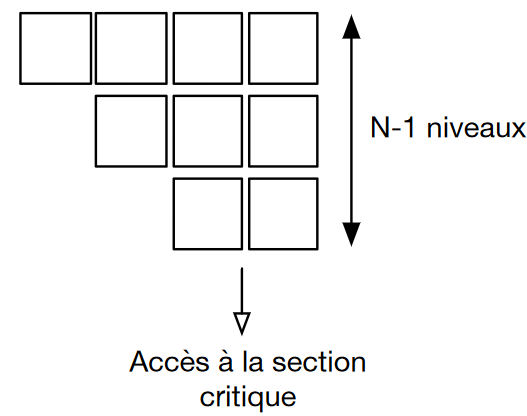
\includegraphics{image-25.png}
\caption{Alt text}
\end{figure}

Si des threads veulent passer il faut que: - Au moins 1 passe - Au moins
1 reste

Quand on est au dernier niveau avec 2 threads, un des deux passe et
l'autre attend.

Pour mettre cela en oeuvre, un thread qui annonce qu'il rentre dans un
nouveau niveau va laisser passer les autres d'abord.

On a 2 tableaux partagés. 1. \texttt{level{[}N{]}}: indexé par le
\textbf{numéro de Thread} et indique son niveau 2.
\texttt{victim{[}N{]}}: indexé par le \textbf{niveau} et dit quel thread
est en attente.

\begin{Shaded}
\begin{Highlighting}[]
\CommentTok{// Thread i}
\CommentTok{// Parcours des niveaux 1 à n{-}1}
\ControlFlowTok{for} \OperatorTok{(}\DataTypeTok{int}\NormalTok{ L }\OperatorTok{=} \DecValTok{1}\OperatorTok{;}\NormalTok{ L }\OperatorTok{\textless{}}\NormalTok{ N}\OperatorTok{;}\NormalTok{ L}\OperatorTok{++)} \OperatorTok{\{}
    \CommentTok{// Annoncer l\textquotesingle{}intention de rentrer au niveau L}
\NormalTok{    level}\OperatorTok{[}\NormalTok{i}\OperatorTok{]} \OperatorTok{=}\NormalTok{ L}\OperatorTok{;}
    \CommentTok{// Le thread se désigne comme la victime pour ce niveau}
\NormalTok{    victim}\OperatorTok{[}\NormalTok{L}\OperatorTok{]} \OperatorTok{=}\NormalTok{ i}\OperatorTok{;}
    \CommentTok{// Attendre tant qu\textquotesingle{}il existe au moins un thread au même niveau ou à un}
\NormalTok{    niveau supérieur}\OperatorTok{,}
    \CommentTok{// et que le thread i est la victime du niveau où il se trouve}
    \DataTypeTok{int}\NormalTok{ t\_niv\_sup\_egal }\OperatorTok{=} \DecValTok{0}\OperatorTok{;}
    \ControlFlowTok{do} \OperatorTok{\{}
    \ControlFlowTok{for} \OperatorTok{(}\DataTypeTok{int}\NormalTok{ j}\OperatorTok{=}\DecValTok{0}\OperatorTok{;}\NormalTok{ j}\OperatorTok{\textless{}}\NormalTok{ N}\OperatorTok{;}\NormalTok{ j}\OperatorTok{++)} \OperatorTok{\{}
        \CommentTok{// parcours du tableau des niveaux pour déterminer si un thread}
        \CommentTok{// est au même niveau ou à un niveau supérieur}
        \ControlFlowTok{if} \OperatorTok{((}\NormalTok{j}\OperatorTok{!=}\NormalTok{i}\OperatorTok{)} \OperatorTok{\&\&}\NormalTok{ level}\OperatorTok{[}\NormalTok{j}\OperatorTok{]} \OperatorTok{\textgreater{}=}\NormalTok{L}\OperatorTok{)} \OperatorTok{\{}
\NormalTok{            t\_niv\_sup\_egal }\OperatorTok{=} \DecValTok{1}\OperatorTok{;}
        \OperatorTok{\}}
    \OperatorTok{\}}
    \OperatorTok{\}} \ControlFlowTok{while} \OperatorTok{(}\NormalTok{t\_niv\_sup\_egal }\OperatorTok{\&\&}\NormalTok{ victim}\OperatorTok{[}\NormalTok{L}\OperatorTok{]==}\NormalTok{i}\OperatorTok{);}
\OperatorTok{\}}
\NormalTok{section\_critique}\OperatorTok{();}
\CommentTok{// Libération de threads bloqués en attente dans les niveaux inférieurs}
\NormalTok{level}\OperatorTok{[}\NormalTok{i}\OperatorTok{]=}\DecValTok{0}\OperatorTok{;}
\end{Highlighting}
\end{Shaded}

Si on décompose le code, on voit qu'un thread progresse si: - Il n'y
aucun thread en attente à son niveau - Il y a un autre thread qui a pris
le rôle de victime.

Au plus N-L threads peuvent dépasser le niveau L. Donc au plus 1 seul
thread peut accéder au niveau N-1.

\begin{figure}
\centering
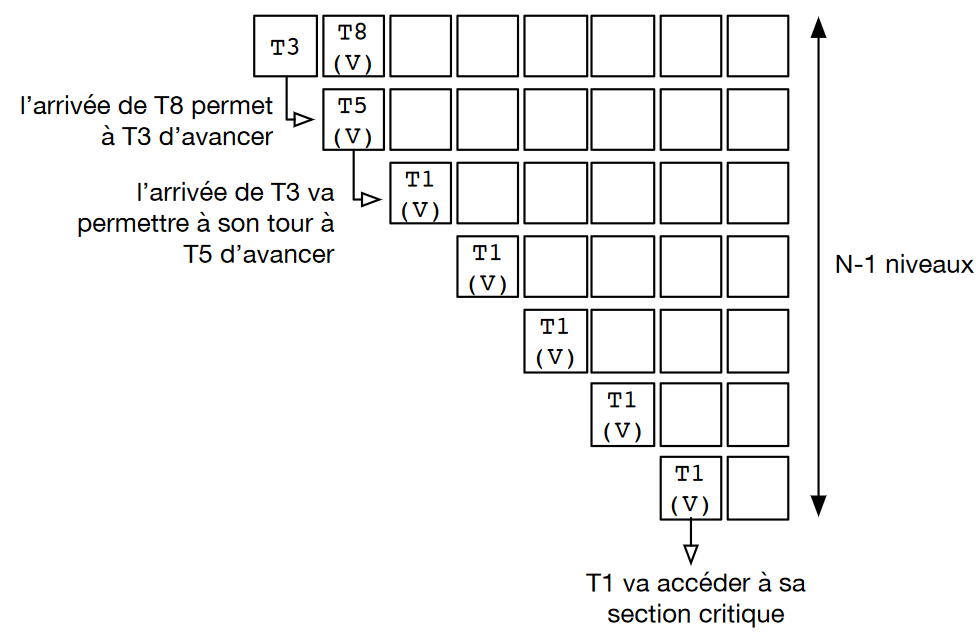
\includegraphics{image-26.png}
\caption{Alt text}
\end{figure}

\subsubsection{Équité}\label{uxe9quituxe9}

On n'a pas la garantie qu'un thread arrivé en premier tout au-dessus des
niveaux va s'exécuter que ceux arriver ! Cela dépend du temps alloué par
le processeur et ce cas de figure ci peut se passer:

\begin{figure}
\centering
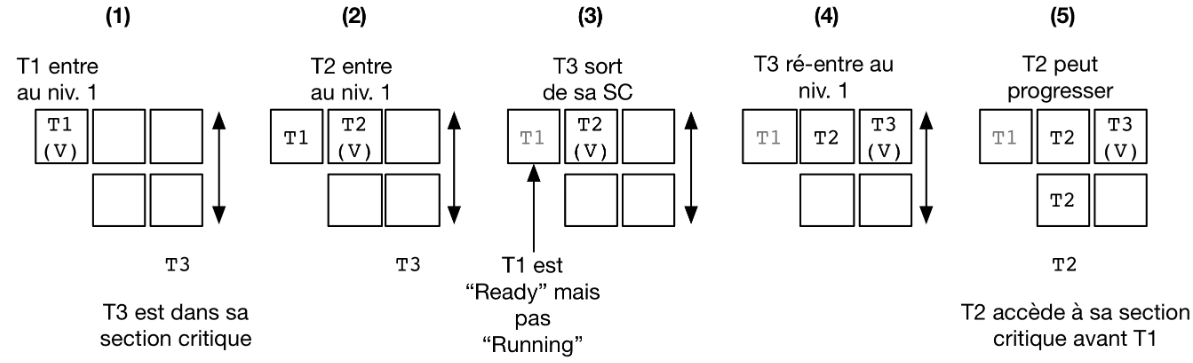
\includegraphics{image-27.png}
\caption{Alt text}
\end{figure}

Ceci arrive à partir de 3 threads.

On peut donc définir l'équité et rendre l'algorithme plus équitable
(permettant d'assurer la propriété de \textbf{liveness}). On va
subdiviser en 2 la partie d'accès à la section critique: 1.
\emph{Doorway}: en un nombre de pas borné, configuration de variables
partagées 2. \emph{Waiting}: boucle \texttt{while()} qui vérifie une
condition.

Garantie formelle d'équité : si la section doorway \(D_A\) d'un thread
\(T_A\) termine avant le début de la section doorway \(D_B\) d'un thread
\(T_B\), alors \(T_A\) a la garantie d'accéder à sa section critique
avant \(T_B\).

À savoir qu'on peut avoir une exécution concurrente de \(D_A\) et
\(D_B\) et donc l'ordre peut être arbitraire. On peut aussi avoir le
\emph{k-bounded waiting} donc pas plus de k sections critiques de
différences entre deux threads. FIFO c'est un 1-bounded waiting.

\subsection{Bakery Algorithm}\label{bakery-algorithm}

Se base sur les tickets de boucherie. On doit toujours savoir combien de
threads on a à l'avance. On a également 2 tableaux partagées: 1.
\texttt{drapeau{[}N{]}}: indexé par le \textbf{numéro du Thread} et
indique s'il veut rentrer en SC. 2. \texttt{ticket{[}N{]}}: indexé par
le \textbf{numéro du Thread} et indique le numéro dans la file.

\textbf{HYPOTHÈSES:} On a également des sections \textbf{doorway} qui ne
sont jamais concurrentes. On aura jamais 2 threads avec le même numéro
de ticket.

C'est \textbf{complètement} irréaliste de penser cela !! Par exemple, 2
threads peuvent observer le même état et donc prendre le même numéro de
ticket !

Donc on doit juste définir un \textbf{ordre de passage} pour les threads
ayant le même numéro ! Le plus simple est de prendre le thread avec le
plus petit numéro.

\begin{Shaded}
\begin{Highlighting}[]
\CommentTok{// Thread i}
\CommentTok{// Section doorway : annoncer son intérêt et obtenir un ticket}
\NormalTok{drapeau}\OperatorTok{[}\NormalTok{i}\OperatorTok{]=}\DecValTok{1}\OperatorTok{;}
\DataTypeTok{int}\NormalTok{ t}\OperatorTok{=}\DecValTok{0}\OperatorTok{;}
\CommentTok{// Parcours des tickets}
\ControlFlowTok{for} \OperatorTok{(}\DataTypeTok{int}\NormalTok{ j}\OperatorTok{=}\DecValTok{0}\OperatorTok{;}\NormalTok{ j}\OperatorTok{\textless{}}\NormalTok{N}\OperatorTok{;}\NormalTok{ j}\OperatorTok{++)} \OperatorTok{\{}
    \ControlFlowTok{if} \OperatorTok{(}\NormalTok{ticket}\OperatorTok{[}\NormalTok{j}\OperatorTok{]\textgreater{}}\NormalTok{t}\OperatorTok{)} \OperatorTok{\{}
\NormalTok{        t }\OperatorTok{=}\NormalTok{ ticket}\OperatorTok{[}\NormalTok{j}\OperatorTok{];}
    \OperatorTok{\}}
\OperatorTok{\}}

\CommentTok{// Prise du ticket supérieur}
\NormalTok{ticket}\OperatorTok{[}\NormalTok{i}\OperatorTok{]=}\NormalTok{t}\OperatorTok{+}\DecValTok{1}\OperatorTok{;}
\CommentTok{// Section waiting : attendre son tour ...}

\ControlFlowTok{do} \OperatorTok{\{}
    \DataTypeTok{int}\NormalTok{ mon\_tour }\OperatorTok{=} \DecValTok{1}\OperatorTok{;}
    \CommentTok{// Parcours des tickets des autres threads dont le drapeau est levé}
    \ControlFlowTok{for} \OperatorTok{(}\DataTypeTok{int}\NormalTok{ j}\OperatorTok{=}\DecValTok{0}\OperatorTok{;}\NormalTok{ j}\OperatorTok{\textless{}}\NormalTok{N}\OperatorTok{;}\NormalTok{ j}\OperatorTok{++)} \OperatorTok{\{}
        \ControlFlowTok{if} \OperatorTok{(}\NormalTok{drapeau}\OperatorTok{[}\NormalTok{j}\OperatorTok{])} \OperatorTok{\{}
            \ControlFlowTok{if} \OperatorTok{((}\NormalTok{ticket}\OperatorTok{[}\NormalTok{j}\OperatorTok{]} \OperatorTok{\textgreater{}}\NormalTok{ ticket}\OperatorTok{[}\NormalTok{i}\OperatorTok{])} \OperatorTok{||} \OperatorTok{((}\NormalTok{ticket}\OperatorTok{[}\NormalTok{j}\OperatorTok{]==}\NormalTok{ticket}\OperatorTok{[}\NormalTok{i}\OperatorTok{])} \OperatorTok{\&\&}\NormalTok{ j}\OperatorTok{\textgreater{}}\NormalTok{i}\OperatorTok{))} \OperatorTok{\{}
            \CommentTok{// Il y a un autre thread actif devant dans la file ...}
\NormalTok{                mon\_tour }\OperatorTok{=} \DecValTok{0}\OperatorTok{;}
            \OperatorTok{\}}
        \OperatorTok{\}}
    \OperatorTok{\}}
\OperatorTok{\}} \ControlFlowTok{while} \OperatorTok{(!}\NormalTok{mon\_tour}\OperatorTok{);}

\NormalTok{section\_critique}\OperatorTok{();}
\CommentTok{// Libération de threads en attente avec les tickets suivants}
\NormalTok{drapeau}\OperatorTok{[}\NormalTok{i}\OperatorTok{]=}\DecValTok{0}\OperatorTok{;}
\end{Highlighting}
\end{Shaded}

Ici, on utilise que des lecteurs écrivains pour mettre en place les
threads. On ne communique pas au \emph{scheduler} ce qui est mis en
pause. Ce n'est pas très optimal car on risque de donner de la ressource
à un thread qui ne peut progresser.

On pourrait faire des opérations sur le processeur pour palier à ça mais
ça ne va pas fonctionner ! En effet, l'ordinateur va ré-arranger les
instructions et les optimiser donc l'ordre d'exécution n'est pas
garanti.

Utiliser le mot-clé \texttt{volatile} pour forcer le programme à relire
tout le temps la valeur ne va pas non plus résoudre le problème à cause
des ordres d'exécution ``\emph{aléatoires}''. (Il existe des barrières
pour forcer des contraintes d'accès à la mémoire \texttt{MFENCE},
\texttt{LFENCE} et \texttt{SFENCE})

On va préférer utiliser des opérations atomiques

\section{Utilisation des Opérations
Atomiques}\label{utilisation-des-opuxe9rations-atomiques}

Une opération est: \emph{une opération qui ne peut être interrompue par
l'arrivée d'une interruption}. On réalise cela via un registre et un mot
mémoire. Les opérations sont donc exécutées de manière
\textbf{séquentielle}.

\subsection{\texorpdfstring{Instructions
\texttt{xchg}}{Instructions xchg}}\label{instructions-xchg}

\begin{Shaded}
\begin{Highlighting}[]
\NormalTok{xchgl \%eax, (var) }
\end{Highlighting}
\end{Shaded}

Équivalent:

\begin{Shaded}
\begin{Highlighting}[]
\NormalTok{movl (var), \%ebx}
\NormalTok{movl \%eax, (var)}
\NormalTok{movl \%ebx, \%eax}
\end{Highlighting}
\end{Shaded}

On a une exclusion mutuelle en utilisant simplement un unique mot
mémoire partagée (ils vont donc tenter d'écrire dans une variable lock 1
qui était libre 0).

\subsubsection{Exclusion Mutuelle}\label{exclusion-mutuelle}

Après un appel à un \texttt{xcgh} il y a deux possibilités: 1.
\texttt{\%eax} contient 0 : l'adresse (\texttt{lock}) a été mise de 0 à
1. * Donc est maintenant réservé et le thread peut rentrer en SC. 2.
\texttt{\%eax} contient 1 : l'adresse (\texttt{lock}) a été mise à 1
mais valait déjà 1 avant l'appel ! * Donc le \texttt{lock} n'était pas
libre ! On va donc boucler et ré-essayer

C'est une approche \emph{test-and-set}.

\subsubsection{Attente Active
(spinlocks)}\label{attente-active-spinlocks}

Les algorithmes basées sur une boucle \texttt{while} qui check une
condition à chaque fois sont appelés des algorithmes \emph{spinlocks}.

Cela fait du travail inutile pour le processeur. Vraiment problématique
pour du code sur mono-coeur car c'est inutile !

\subsubsection{Mutex POSIX}\label{mutex-posix}

On va ici utiliser le support du \textbf{Système d'Exploitation}. Si un
thread veut faire un \texttt{lock()} sur un mutex \emph{déjà bloqué}
alors ce thread sera mis en état \textbf{blocked}. Il est maintenant
dans une file d'attente pour que le mutex soit \texttt{unlock()}.

\textbf{Avantages:} On perd pas de ressources inutilement. Utile pour
gérer les sections critiques.

\textbf{Inconvénients:} On a une grande latence entre l'appel
\texttt{lock()} et l'exécution de la section critique.

\paragraph{Comparaison}\label{comparaison}

\textbf{Attente active} que sur multi-processeur. Utile pour les
sections critiques courtes. Fort utilisé dans le noyau !

\textbf{Mutex} plus efficace pour mettre en oeuvre la synchronisation
avec équité. On ne schedule pas des threads non prioritaires avant ceux
qui doivent accéder à leur SC en premier.

\subsection{\texorpdfstring{Test-and-set
\texttt{xchg}}{Test-and-set xchg}}\label{test-and-set-xchg}

Si on utilise cet algorithme avec un \texttt{xchg} c'est
\textbf{catastrophique}. On a une latence d'accès au sections critiques
qui augmentent avec le nombre de threads.

Ceci est causé par le \textbf{cache} !

\begin{figure}
\centering
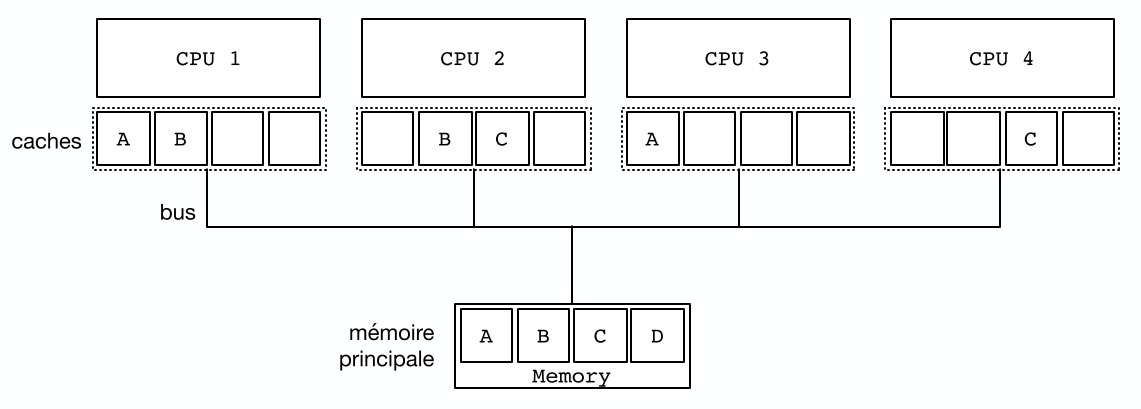
\includegraphics{image-28-1.png}
\caption{Alt text}
\end{figure}

On a donc un cache pour chaque coeur et les adresses mémoires récemment
utilisées. Mais on a aucun moyen de s'assurer de la cohérence du tout.

\subsubsection{Utilisation du Cache}\label{utilisation-du-cache}

On utilise donc le \emph{bus} pour coordonner la mise à jour et
l'invalidation de leur contenu.

On a chaque contrôleur qui \emph{snoop} le bus. Un seul contrôleur peut
utiliser le bus à un moment. La mémoire va donc écouter le bus et
répondre aux requêtes de lecture/écriture.

\subsubsection{Protocole de Cohérence de Cache
MSI}\label{protocole-de-cohuxe9rence-de-cache-msi}

Chaque ligne de cache a donc 3 états: - \textbf{M} \emph{modified}: la
valeur en cache est plus récente que celle en mémoire principale. -
\textbf{S} \emph{shared}: lignes présentes à d'autres endroits et
identiques. - \textbf{I} \emph{invalid}: on ne peut pas utiliser cette
ligne. L'accès doit retourner vers le bus pour avoir la version la plus
à jour.

\begin{figure}
\centering
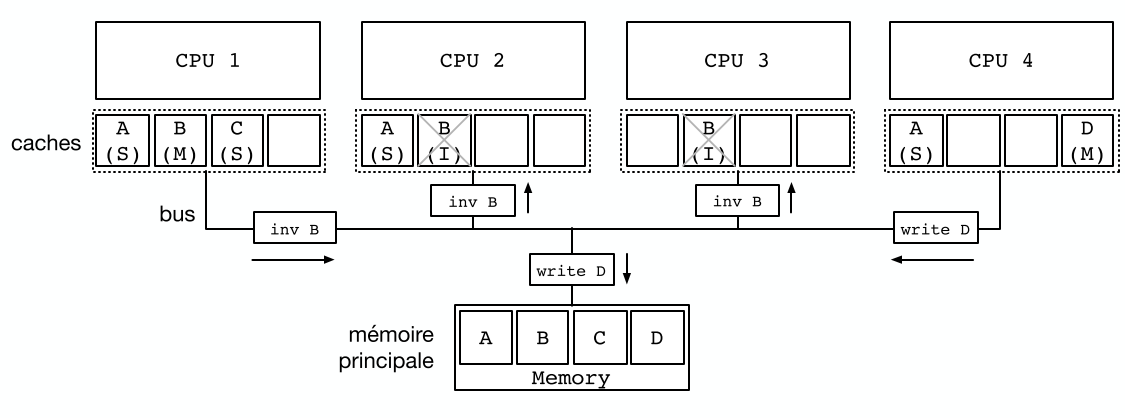
\includegraphics{image-29-1.png}
\caption{Fonctionnement MSI}
\end{figure}

Donc pour écrire une ligne en mode S, le contrôleur de cache doit
invalider les autres copies de S et passer la ligne en mode M.

Avec cela, on peut assister à un phénomène de ping-pong entre les caches
si deux threads s'exécutent sur des processeurs différents. À chaque
modification, un des deux threads doit invalider la valeur chez l'autre
et modifier le tout.

Le \textbf{faux partage} arrive lorsque deux variables distinctes sont
dans la même ligne de cache.

\subsubsection{Instructions Atomiques \& Utilisation du
Bus}\label{instructions-atomiques-utilisation-du-bus}

Avec un \texttt{xchg}, on doit avoir accès à la ligne de cache en mode
\textbf{M} mais aussi assurer qu'aucune opération concurrente ne soit
possible. Il faut verrouiller le bus le temps de l'exécution.

Donc il y a un coup pour le processeur qui l'exécute pour assurer
l'atomicité mais aussi pour les autres car ils ne peuvent plus rien
exécuter.

Donc on va saturer via un test-and-set le bus de message d'invalidation
et en le bloquant.

\paragraph{Solution:
test-and-test-and-set}\label{solution-test-and-test-and-set}

On tire profit que tant que la variable \texttt{lock} est à 1, le thread
\(T_A\) exécute sa section critique. On va éviter de faire des appels à
\texttt{xchg}. Tant que \texttt{lock} est à 1 on peut faire une lecture
depuis le cache et si on lit 0 alors il tente d'appeler \texttt{xchg}.

\begin{Shaded}
\begin{Highlighting}[]
\ControlFlowTok{while} \OperatorTok{(}\NormalTok{test\_and\_set}\OperatorTok{(}\NormalTok{verrou}\OperatorTok{,} \DecValTok{1}\OperatorTok{))} \OperatorTok{\{} 
    \CommentTok{// on a pas obtenu le verrou car on a lu 1 }
    \CommentTok{// donc on attend de lire 0 pour tenter à nouveau while (verrou) \{\}}
\OperatorTok{\}}
\end{Highlighting}
\end{Shaded}

\begin{figure}
\centering
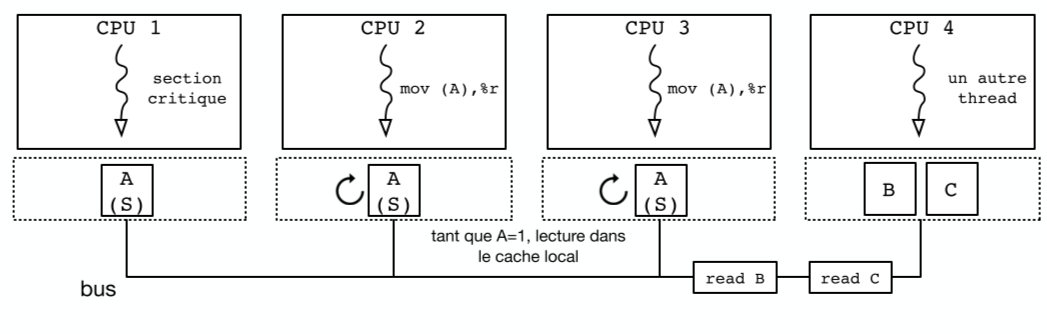
\includegraphics{image-30-1.png}
\caption{Alt text}
\end{figure}

Cela va réduire sensiblement le traffic et l'immobilisation du bus quand
la contention est élevée. Mais cela impact toujours de manière non
négligeable.

Dès que \texttt{lock} est libéré tous les autres threads se jettent pour
appeler \texttt{xchg}. Des essais infructueux a de lourds impacts sur le
système. Cela augmente la contention.

\paragraph{backoff-test-and-test-and-test}\label{backoff-test-and-test-and-test}

On peut aussi attendre et revenir plus tard !

Si lors d'un second essai la contention est toujours forte on va
attendre encore plus longtemps. On adapte les ressources nécessaires en
fonction du trafic.

On va souvent utiliser du \textbf{exponentiel-backoff}. Si on arrive pas
du premier coup, on va attendre un temps aléatoire entre
\texttt{{[}0:v{]}} avec \(v=v_{init}\). Au deuxième essai, on attendra
\(v=v*2\) et cela jusqu'à \(v_{max}\) et on ne doit pas utiliser d'appel
système pour l'attente.

\subsection{Conclusion}\label{conclusion}

\begin{itemize}
\tightlist
\item
  Le problème fondamental à résoudre pour construire des primitives de
  synchronisation est celui de l'exclusion mutuelle

  \begin{itemize}
  \tightlist
  \item
    Avec des garanties de liveness : pas de \emph{livelock} ou
    d'hypothèses sur l'entrelacement des opérations
  \end{itemize}
\item
  Algorithmes classiques difficiles à utiliser sur les architectures
  modernes car fondés sur des hypothèses sur l'ordre des accès mémoire
  et une utilisation de la mémoire en \(O(N)\)
\item
  Utilisation d'instructions atomiques pour résoudre l'exclusion
  mutuelle avec \(O(1)\) mot partagé
\item
  Attention à la mise en oeuvre et à l'impact sur le cache et la
  performance !
\end{itemize}
